\chapter{Introduction}

\section{Motivation}
Traditional approaches to data collection often rely on extensive experiments using full-scale systems, such as MilliAmpere, which is an autonomous surface vehicle developed at NTNU \cite{brekkeMilliAmpereAutonomousFerry2022}.
While these experiments are crucial for specific research purposes, the cost-benefit ratio may not be favorable when the primary objective is to collect sensor data.

The absence of a low-threshold approach to data collection was identified together with my supervisors at the beginning of my integrated Ph.D.
To address this, I started developing a human-operable sensor rig during my \preproject, aiming to complete it during my \master.
The overarching goal was to create a lightweight \sr that could overcome typical challenges like synchronization and pose estimation, paving the way for an accessible approach to low-effort acquisition of high-quality data.

While significant progress was made in the mechanical design and electronic aspects during my \preproject, considerable work remained on the software side to make the \sr fully operational.
Three main goals were set for this \master:

\subsection{Integration of Polarization Cameras}
Although the \sr platform is designed to support various sensors, this \master project primarily focuses on integrating two polarization cameras from \lucid.
These cameras capture information about the polarization state of the incoming light in addition to color information.
Their utility is particularly advantageous in maritime environments, as light reflected on the water surface has characteristic polarization properties.

\subsection{High Speed Video Acquisition and On-the-Fly Compression}
\label{sec:intro:compression}
Much work was put into enabling on-the-fly compression of the video streams from the \sr.
Each \cam on the \sr features a 5.0MP sensor configured to capture 10-bit raw images 16 times every second, resulting in roughly $1Gb/s$ of data \cite{lucidvisionlabsTriton0MPPolarization}.
To put this into perspective, a single frame contains more data than is needed to store the entire collection of William Shakespeare's works in plain text \cite{projectgutenbergCompleteWorksWilliam1994}.
If the output from these cameras were stored directly to disk, almost a Terabyte of data would be generated every hour, making collecting long-term data sets infeasible.

Buying an $8TB$ \gls{ssd} would enable 9 hours of recording, but several arguments for allowing on-the-fly compression remained \cite{CorsairMP600PRO}:

\paragraph{Limited Write Speed to the SSD} currently makes writing all the raw data directly to the \gls{ssd} infeasible.
Even though the installed \gls{ssd} is more than capable, the write speeds were measured just below $2Gb/s$
\footnote{Tested with \code{sudo dd if=/dev/zero of=./testfile bs=8k count=100k conv=fdatkasync}.}
\cite{microntechnologyMicron2300SSD2020}.
Other people have faced similar issues on the \jx \cite{dtyuImbalancedPerformanceRead2018}.
Buying a faster \gls{ssd} might solve this issue, but other arguments remain.

\paragraph{Streaming to External Devices} is another argument for enabling video compression.
The implemented compression pipeline permits separate compression at a higher bit rate for streaming to external devices over WiFi or 4G.

\paragraph{Integration with Other Systems} is easier when the data rate is kept below $1Gb/s$ as it can be transferred over regular ethernet.
The primary intended purpose for the \sr is to be used as a standalone system for data acquisition.
However, the design process has still been guided by the goal of making it easy to integrate with other systems.

\subsection{Graphical Web Interface and Ergonomic Improvements}
The ultimate objective for the \sr is to make data acquisition as easy as possible.
Given the significant effort invested, ensuring user-friendliness was essential to maximize the utilization of the \sr.
A graphical web interface was developed to enable real-time control and monitoring of the \sr from a mobile device.
This eliminates the requirement for SSH access and transforms the \sr into a plug-and-play system.

In addition to the web interface, several ergonomic improvements were made to the hardware design, making it easier to carry and operate the \sr.

\begin{figure}[H]
    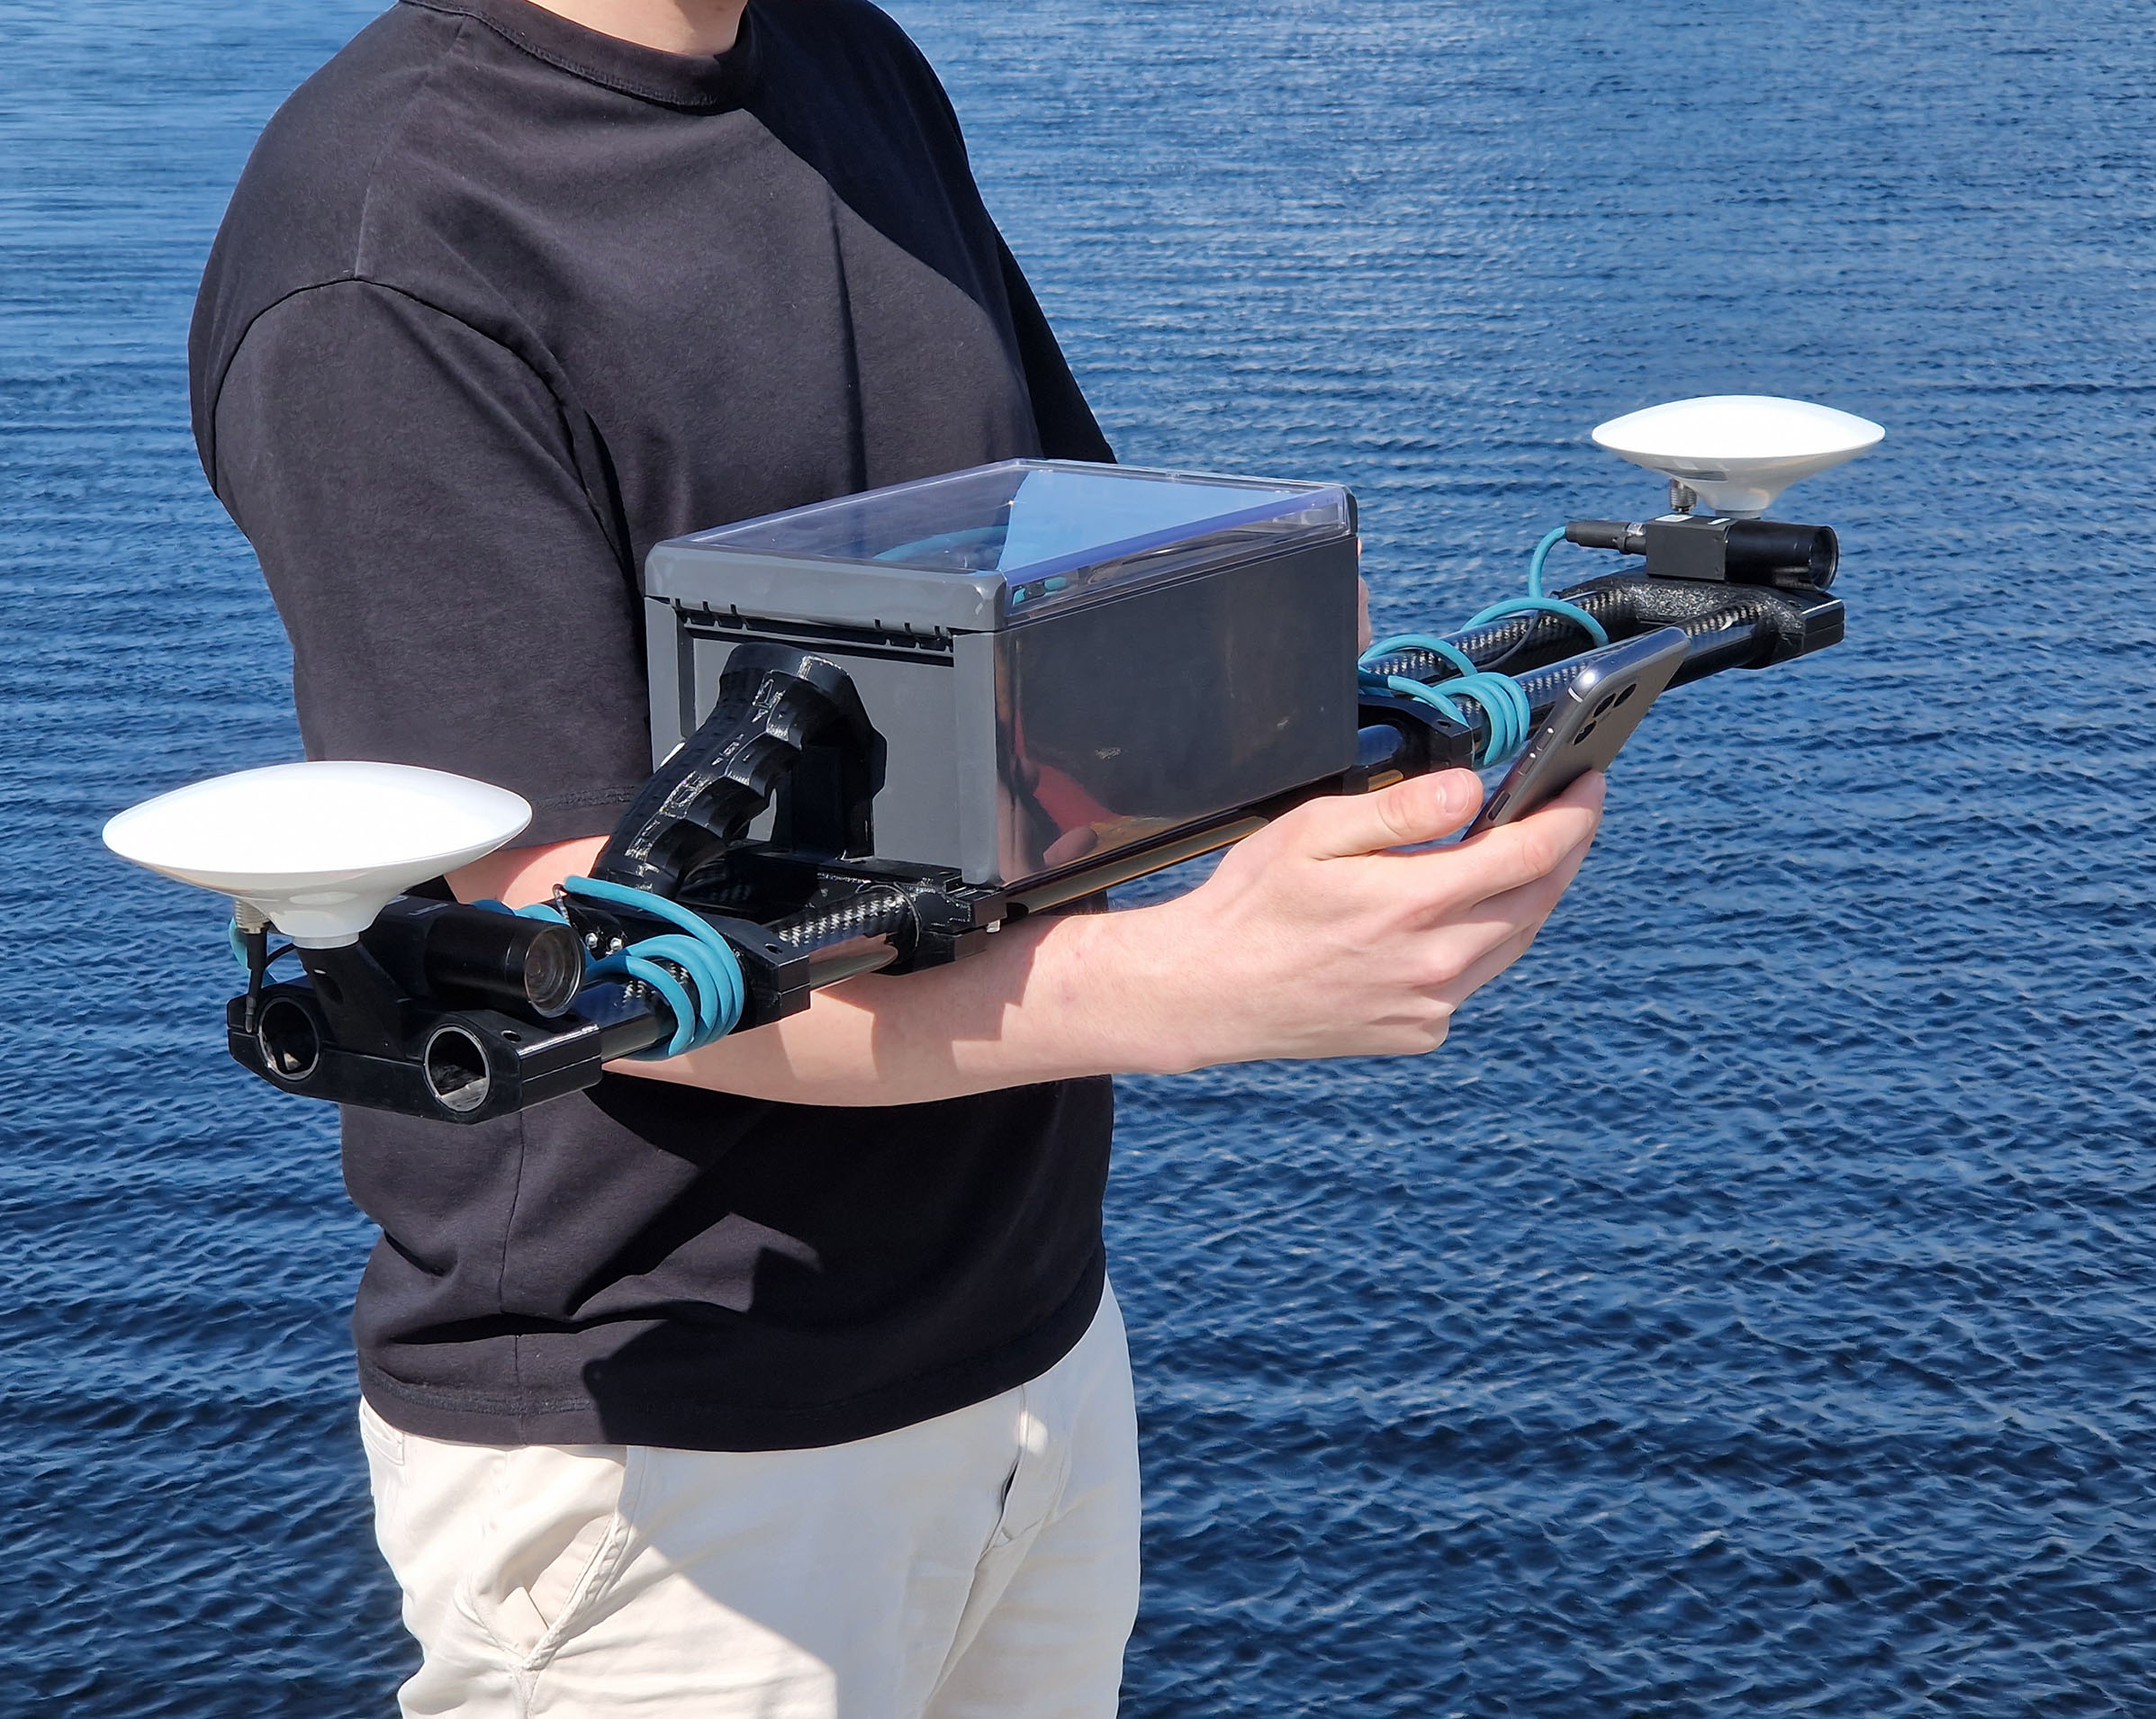
\includegraphics[width=\textwidth]{figures/frontpage.jpg}
    \caption{The Sensor Rig}
\end{figure}

\section{Previous Work}
This \master is an extension of the work in my \preproject \cite{martensPortableSensorRig2022}.
During the \preproject I finished most of the hardware design of the \sr
and assembled the necessary electronics for \gls{spi} communication between the \jx and the \gls{navbox}, which is the small assembly containing the \gls{imu} and the \gls{gnss} receivers.

At the end of the \preproject the \sr was capable of collecting data from the \gls{imu} and the \glspl{gnss} and validating the \gls{crc} checksum on the incoming data.
I had verified that it was possible to read data from the \cams over the ethernet interface, but only at a very low framerate using the default settings.

As this \master is closely related to the \preproject it will reference several sections and figures to avoid having to repeat wats already written there, and the reader is advised to have it available.

\section{Main Contributions}
The main contribution of this \master is the delivery of a working \sr capable of recording high-quality stereo polarization datasets.
In terms of specific technical achievements, the following are the main contributions:

\begin{itemize}
    \item Developed and implemented a higly efficient \gls{cuda} kernel transforming the raw output from the \cams into the widly used \gls{p010} format.
    \item Assembled a \py acessible \gls{gstreamer} pipeline for hardware acceleraded compression on the \jx.
    \item Developed a full-stack graphical web interface accessible from mobile devices.
    \item Designed and 3D-printed ergonomic handles for the \sr.
\end{itemize}


\section{Outline}
Completing the \sr project has involved extensive work on various topics, ranging from hardware design and full-stack web development to kernel compilation and low-level optimizations in \gls{cuda}{cuda}.
Although some topics are closely related, others are only connected by contributing towards the final product.

With this in mind, it has been difficult to decide on a structure for this report and what to include.
In the end, I decided to collect the software development theory in the first chapter and dedicate a chapter to each of the major topics I have worked on, with a focus on the practical aspects of the work.

As some chapters might be less relevant depending on the reader's background, I have tried to make each chapter as self-contained as possible.
Figure \ref{fig:overview} provides an overview of the chapters in this \master and how they are connected.
Following is a brief introduction to each chapter:

\begin{figure}[H]
    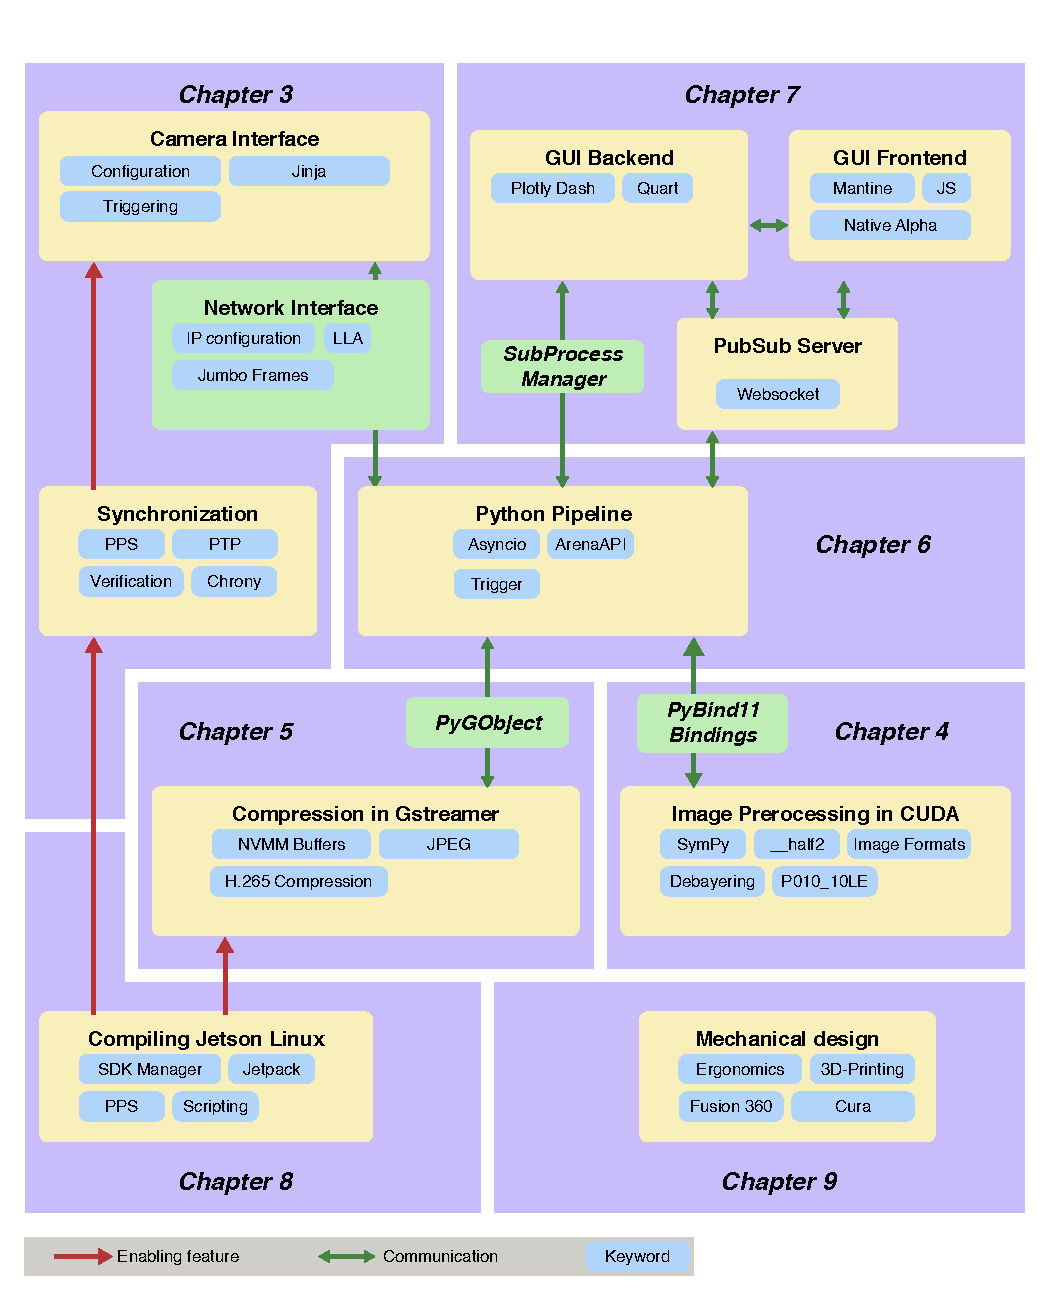
\includegraphics[width=\textwidth]{chapters/10_intro/chapter_overview.pdf}
    \caption{Overview of the chapters in this \master.}
    \label{fig:overview}
\end{figure}


\paragraph{Chapter \ref{chap:programming_theory}: Real time programming on Jetson Xavier}
This chapter provides an overview of the theoretical background relevant to real-time performance on the Jetson Xavier platform and the development of real-time software in general.
It explores performance considerations for heterogeneous systems and introduces the \gls{cuda} programming model.

\paragraph{Chapter \ref{chap:cameras}: Polarization Cameras}
This chapter presents the special type of polarization cameras used, explains how they work, and why they are particularly well suited for detection in marine environments.
Furthermore, it covers how to interact with the \cams through their \gls{api} and how the network adapters have been configured to achieve reliable $2Gb/s$ throughput from the \cams.

\paragraph{Chapter \ref{chap:debayer}: Efficient Preprocessing of Raw Image Data in CUDA}
To make it possible to compress the video streams, the raw data has to be transformed into a format that can be processed by the \gls{h265} encoder.
This chapter explains how this is achieved in real-time using \gls{cuda}.

\paragraph{Chapter \ref{chap:gstreamer}: Video Compression using GStreamer}
\gls{gstreamer} is a powerful framework for processing video streams.
This chapter explains how it is used to compress the video streams in real-time using hardware acceleration on the \jx.
It also covers how \gls{pygo} is used to interact with the \gls{gstreamer} pipeline from Python.

\paragraph{Chapter \ref{chap:pipeline}: Pipeline Assembly in Python}
This chapter links the preceding three chapters, illustrating assembling the different components into a functional pipeline.
An outline of the pipeline's operation and a discussion on certain design choices is presented.

\paragraph{Chapter \ref{chap:gui}: Web Interface to Control, Monitor and Stream Video}
This chapter presents the web application developed to enable real-time control and monitoring of the \sr and its video streams.
The application allows anyone with a smartphone to operate the \sr without any prior training or technical knowledge.
In addition, a \gls{pubsub} server has been implemented for communication between the web application and the pipeline.

\paragraph{Chapter \ref{chap:flashing_xavier}: Compiling Jetson Linux with PPS Enabled}
This chapter presents a systematic approach to compile, flash and debug the \gls{os} on the \jx.
Updating the \gls{os} was necessary to get the \gls{gstreamer} pipeline working.
As \gls{pps} support is required to synchronize the clock on the \jx to \gls{utc}, it was necessary to configure the underlying Linux kernel to support this, which was more complicated than expected.

\paragraph{Chapter \ref{chap:hardware}: Improving Ergonomics and Mechanical Rigidity}
After the \preproject most of the hardware was already in place, but some parts were missing.
I applied for funding and purchased a new 3D printer to enable an iterative design process.
With this in place, custom ergonomic carry handles, new combined camera and antenna mounts, and other minor parts were designed and 3D-printed.

\paragraph{Chapter \ref{chap:results}: Results}
With everything in place, the \sr was tested in the field.
Several smaller datasets are collected, and visualization tools have been developed to facilitate the analysis of the data.

\paragraph{Chapter \ref{chap:future_work}: Ongoing developments and future work}
Some design flaws from the \preproject remain to be fixed, and a few possible performance improvements have been identified.
With the goal of creating a fully autonomous sensor rig achieved, the next step is to create state-of-the-art stereo polarization datasets and advance the field of situational awareness for autonomous surface vessels.

